\section{A Design Process for Complete Dynamic System Design\label{sec:ch1:process}}

\begin{figure}
\centering
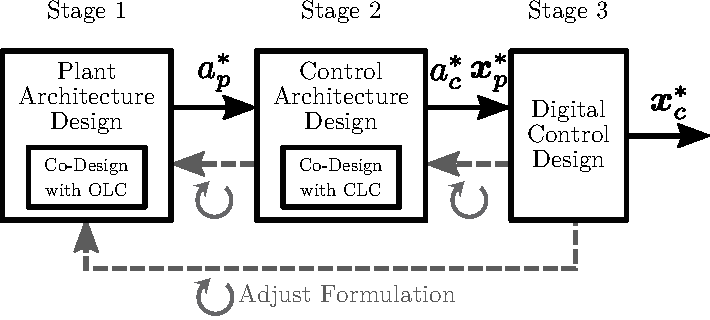
\includegraphics[width=0.6\textwidth]{../ch1/figures/stages2.pdf}
\caption{Proposed stages for complete dynamic system design.\label{fig:ch1:stages}}
\end{figure}

Allowing flexibility in all design domains can create a number of challenges that can limit how effectively one arrives at a suitable solution.
Here we adopt the design process proposed in Ref.~\cite{Deshmukh2015a} for complete dynamic system design that helps manage the complexity and uncertainty found in combined architecture, plant, and control design problems.
It is a three stage process shown in Fig.~\ref{fig:ch1:stages}.
We denote the plant architecture as $\glsfirst{architecture}_{\glsfirst{plant}}$ and associated plant variables as $\gls{x}_p$.
The control architecture is represented with $a_{\glsfirst{control}}$ and control variables $\bm{x}_c$ (and OLC variables as $\gls{olc}$).
The system-level objective function is represented by $\gls{objective}$.

% new paragraph
The first stage seeks to determine the optimal plant architecture by forgoing the specification of the control architecture.
Using a specific control architecture limits creative plant design exploration at early design stages \cite{Deshmukh2015a}.
Instead, OLC is used for the control among other potential uses.
OLC can replace some components or interfaces with optimal trajectories, reducing the design problem size while still providing an optimal solution \cite{Deshmukh2015a, Herber2014a, Allison2014b}.
In addition, OLC-based studies are particularly valuable at early design stages for gaining insights into upper system performance limits and dynamic behaviors and interactions that lead to system-optimal performance \cite{Allison2014a, Allison2013d,Son2010a, Schaala1993a, Mourik2009a, Karkee2010a}.
Furthermore, combined plant and control design, or co-design, will be used to determine the performance for each candidate plant architecture because it is a system-level optimization strategy \cite{Herber2017b, Fathy2003a, Allison2014a} that will allow fair comparisons between candidate plant architectures \cite{Bayrak2015a}.

\begin{figure}
\centering
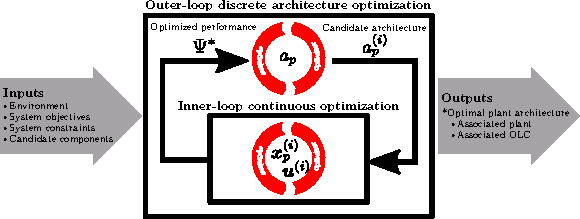
\includegraphics[width=0.8\textwidth]{../ch1/figures/outerinner2.pdf}
\caption{Stage 1 details.\label{fig:ch1:outerinner}}
\end{figure}

% new paragraph
The specifics for stage 1 are shown in Fig.~\ref{fig:ch1:outerinner}.
The inputs are the information about the system's operating environment, objectives, constraints, and a catalog of candidate components.
A nested optimization approach is used to handle the different variable types.
Here the outer loop will change the discrete (plant) architecture design variables while the inner loop determines the optimal performance by solving the continuous co-design problem for the candidate architecture. 

% new paragraph
Stage~2 in Fig.~\ref{fig:ch1:stages} seeks to determine the best control architecture given the optimized plant architecture from stage~1.
Similar to stage~1, a nested optimization approach can be used to vary the discrete control architecture decisions while the appropriate co-design problem is solved to determine the optimal performance for the candidate architecture.
For example, we could consider a basic feedback, hybrid \cite{Lygeros2008a}, or model predictive \cite{Borrelli2017a} controller architectures.
The final stage, stage~3, seeks to determine the digital controller design given the plant and controller architectures from the previous stages \cite{Landau2006a}.

% new paragraph
It might be necessary to iterate between the stages if unforeseen issues appear.
Information about these issues can be passed back to the previous stage and the problem formulation can be adjusted to address overlooked elements.
Additionally, in each of the stages, a sequence of problems may be posed and solved, each one informed by the results of the previous problem, moving toward greater levels of system specificity.

The theory and studies in this dissertation will primarily focus on design problems in stage~1, but it is important to understand the motivations behind these studies and how they fit into the entire design process.